%%%%%%%%%%%%%%%%%%%%%%%%% NOTE %%%%%%%%%%%%%%%%%%%%%%%%%%%%
%% You can ignore everything from here until             %%
%% "Question 1: Introduction"                            %%
%%%%%%%%%%%%%%%%%%%%%%%%%%%%%%%%%%%%%%%%%%%%%%%%%%%%%%%%%%%
\documentclass[8pt]{article}
\usepackage{amsmath, amsfonts, amsthm, amssymb}  % Some math symbols
\usepackage{fullpage}
\usepackage{graphicx}
\usepackage[x11names, rgb]{xcolor}
\usepackage{graphicx}
\usepackage{tikz}
\usetikzlibrary{decorations,arrows,shapes}
\usepackage{float} % Add this package to control float placement
\usepackage{etoolbox}
\usepackage{enumerate}
\usepackage{listings}
\lstset{
    language=Python,           % Set the language of the code
    basicstyle=\footnotesize\ttfamily,
    keywordstyle=\color{blue}, % Set color for keywords
    commentstyle=\color{gray}, % Set color for comments
    stringstyle=\color{red},   % Set color for strings
    numbers=left,              % Display line numbers on the left
    numberstyle=\tiny\color{gray}, % Style for line numbers
    frame=single,              % Add a frame around the code
    breaklines=true            % Allow line breaking
}


\setlength{\parindent}{0pt}
\setlength{\parskip}{5pt plus 1pt}

\newcommand{\N}{\mathbb N}
\newcommand{\E}{\mathbb E}
\newcommand{\V}{Var}
\renewcommand{\P}{\mathbb P}
\newcommand{\f}{\frac}


\newcommand{\nopagenumbers}{
    \pagestyle{empty}
}

\def\indented#1{\list{}{}\item[]}
\let\indented=\endlist

\providetoggle{questionnumbers}
\settoggle{questionnumbers}{true}
\newcommand{\noquestionnumbers}{
    \settoggle{questionnumbers}{false}
}

\newcounter{questionCounter}
\newenvironment{question}[2][\arabic{questionCounter}]{%
    \addtocounter{questionCounter}{1}%
    \setcounter{partCounter}{0}%
    \vspace{.25in} \hrule \vspace{0.4em}%
        \noindent{\bf \iftoggle{questionnumbers}{#1: }{}#2}%
    \vspace{0.8em} \hrule \vspace{.10in}%
}{$ $\newpage}

\newcounter{partCounter}[questionCounter]
\renewenvironment{part}[1][\alph{partCounter}]{%
    \addtocounter{partCounter}{1}%
    \vspace{.10in}%
    \begin{indented}%
       {\bf (#1)} %
}{\end{indented}}

\def\show#1{\ifdefempty{#1}{}{#1\\}}

\newcommand{\header}{%
\begin{center}
    {\Large \show\myhwname}
    \show\myname
    \show\myemail
    \show\mysection
    \show\hwname
\end{center}}

\usepackage{hyperref} % for hyperlinks
\hypersetup{
    colorlinks=true,
    linkcolor=blue,
    filecolor=magenta,      
    urlcolor=blue,
}

%%%%%%%%%%%%%%%%% Identifying Information %%%%%%%%%%%%%%%%%
%% For 312, we'd rather you DIDN'T tell us who you are   %%
%% in your homework so that we're not biased when        %%
%% So, even if you fill this information in, it will not %%
%% show up in the document unless you uncomment \header  %%
%% below                                                 %%
%%%%%%%%%%%%%%%%%%%%%%%%%%%%%%%%%%%%%%%%%%%%%%%%%%%%%%%%%%%
\newcommand{\myhwname}{DS288 (AUG) 3:0 Numerical Methods }
\newcommand{\myname}{Naman Pesricha }
\newcommand{\myemail}{namanp@iisc.ac.in}
\newcommand{\hwname}{\textbf{Homework-2}}
\newcommand{\mysection}{SR - 24115}
%%%%%%%%%%%%%%%%%%%%%%%%%%%%%%%%%%%%%%%%%%%%%%%%%%%%%%%%%%%

%%%%%%%%%%%%%%%%%%% Document Options %%%%%%%%%%%%%%%%%%%%%%
\noquestionnumbers
\nopagenumbers
%%%%%%%%%%%%%%%%%%%%%%%%%%%%%%%%%%%%%%%%%%%%%%%%%%%%%%%%%%%

\begin{document}
\header

\begin{question}{1. Using Newton's method, Secant method, and Modified Newton's method, find the solution of
f(x) = 0 for the functions listed. For the Newton methods start with an initial guess of $p_{0} = 0$.
For the Secant method start with initial guesses (or interval) of $p_{0} = 0$ and $p_{1} = 1$. Iterate until
you reach a relative tolerance of $10^{-6}$ between successive iterates. Report the root found and
the number of iterations needed for each method. \\
(a) $f(x)=x+e^{-x^2}cosx$.\\
(b) $f(x) =(x+e^{-x^2}cosx)^2$.\\
Comment on the observed convergence rates in these cases. Does your results agree with the
analysis we did in class ?. [4 points]}

\textbf{Answer:}\\
\begin{table}[H]
    \centering
    \begin{tabular}{|c|c|c|c|c|c|c|} 
    \hline
         &\multicolumn{2}{|c|}{\textbf{Newtons}}& \multicolumn{2}{|c|}{\textbf{Secant}} & \multicolumn{2}{|c|}{\textbf{Modified Newtons}} \\  
    \hline
    &\textbf{iterations}&\textbf{root} &\textbf{iterations}&\textbf{root} &\textbf{iterations}&\textbf{root} \\
    \hline
         $f(x)=x+e^{-x^2}cosx$& 5 &-0.58840178& 7 &-0.58840178& 6 &-0.58840178	 \\
         $f(x) =(x+e^{-x^2}cosx)^2$& 19 &	-0.58840144& 34 &-0.58840136& 6 &-0.58840178	 \\
    \hline
    \end{tabular}
    \caption{Root values and iterations taken to converge in Newtons. Secant and Modified Newtons methods.}
    \label{tab:my_label}
\end{table}

\begin{figure}[H]
    \centering
    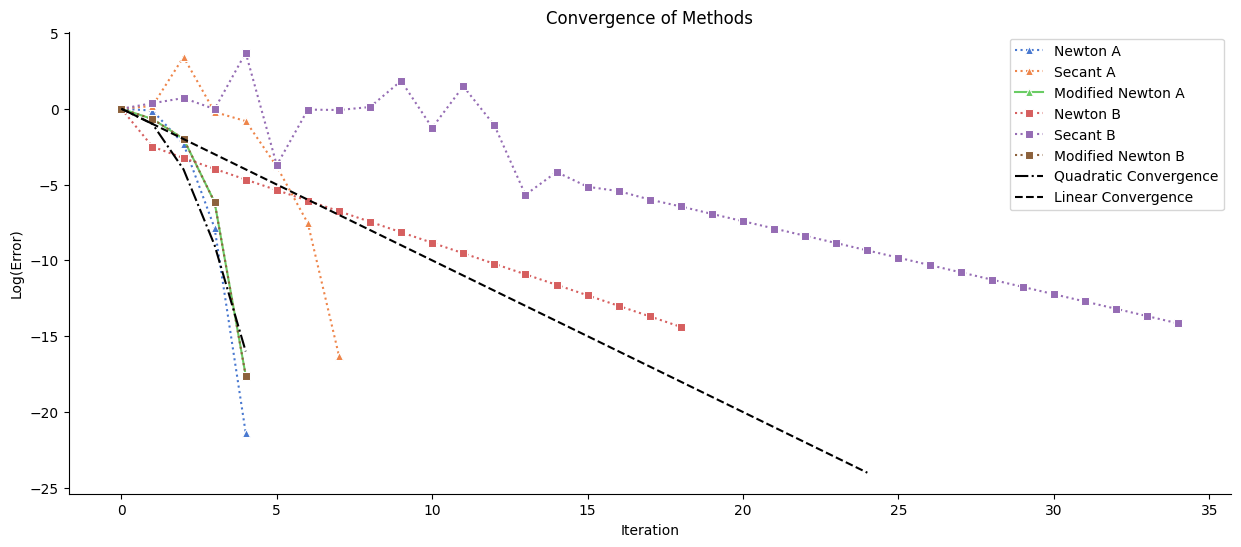
\includegraphics[width=\textwidth]{HW2/convergence.png}
    \caption{Logarithm of error over the iterations.}
    \label{fig:example}
\end{figure}

Problem a) has a single root at $x = -0.588401$\\
Problem b) has root at $x = -0.588401$ with multiplicity 2.

\textbf{From Figure 1, we can make the following observations:}\\
\textbf{1. Newton's Method}: \\
Problem a): Shows better than linear convergence.\\
Reason: Newton's Method has quadratic convergence $\alpha = 2$ for single root problem.\\ \\
Problem b): Shows linear convergence trend. \\ 
Reason: Newton's Method has linear convergence $\alpha = 1$ if root multiplicity $m\geq 2$.\\

\textbf{2. Secant Method}: \\
Problem a): Shows better than linear convergence.\\
Reason: Secant Method has superlinear convergence $\alpha = 1.62$ for single root problem. \\ \\
Problem b): Shows linear convergence trend. \\ 
Reason: Secant Method has linear convergence $\alpha = 1$ if root multiplicity $m\geq 2$.\\

\textbf{3. Modified Newton's Method}: \\
Shows better than linear convergence rate for both problem a) and b).\\
Reason: Modified Newton's Method exhibits quadratic convergence irrespective of root multiplicity. \\

\textbf{4. Newton's Method takes less iterations compared to Secant Method} for problem a) and b) as .

For problem a), since $\alpha_{Newton's \ Method} \geq \alpha_{Secant \ Method}$, and hence Newton's converges in less iterations.

For problem b) the asymptotic error constant of Newtons method is less than that of Secant Method and hence Newton's Method converges in less iterations.

$$\lambda_{Newton's Method} \ < \ \lambda_{Secant Method}$$

In general, for same order of convergence $\alpha$, lower value of $\lambda \implies Faster\ Convergence.$ 
\end{question}

\begin{question}{2. Develop the functional form for a cubicly convergent fixed point iteration function $g(p_{n})$ to solve
the problem f(x) =0 by writing
$$g(x) = x - \phi(x)f(x) - \psi(x)f^2(x)$$
and determining $\phi(x)$ and $\psi(x)$. Specify the asymptotic order of convergence ($\alpha$) and write the
asymptotic error constant ($\lambda$). Write all expressions in terms of $f(p)$ and its derivatives and
simplify your answers. You are allowed to scan the hand-written derivation for this part alone.
Hint: Extend the approach we used in class to derive Newton's method. The scheme you will
produce is often referred to as "Cubic Newton's Method". [3 points]}
For cubic convergence, we want $g'(p) = 0$ and $g''(p) = 0$. We also know that $f(p) = 0$ (if p is the root).

We want to evaluate $\phi(x) | f(x) = 0$ and $\psi(x) | f(x) = 0$.
\begin{equation}
    \fbox{$g(x) = x - \phi(x)f(x) - \psi(x)f^2(x)$}
\end{equation}
$$g'(x) = 1 - \phi'(x)f(x) - \phi(x)f'(x) - \psi'(x)f^2(x) - {2\psi(x)f'(x)f(x)}$$
$$(Subsituting \ g'(x) = 0 \ and \ f(x) = 0)$$
$$1 - \phi(x)f'(x) = 0$$
\begin{equation}
     \textbf{Ans:} \fbox{ $\implies \phi(x) = \frac{1}{f'(x)} \ and \ \phi'(x) = -\frac{f''(x)}{(f'(x))^2}$}
\end{equation}

$$We \ will \ now \ find \ g''(x)$$
$$g'' = \phi''f - \phi'f' - \phi'f' - \phi f'' - \psi''f^2 - 2\psi'f'f - 2\psi' f' f - 2\psi f'' f - 2\psi (f')^2$$

$$(Subsituting \ g''(x) = 0 \ , \ f(x) = 0)$$
$$ - 2\phi'f' - \phi f'' - 2\psi (f')^2 = 0$$

$$(Subsituting \ (2))$$
$$2\frac{f''}{(f')^2}f' - \frac{1}{f'(x)} f'' - 2\psi (f')^2 = 0$$
$$\implies 2\psi (f')^2 = 2\frac{f''}{(f')^2}f' - \frac{1}{f'(x)} f'' $$
$$\implies 2\psi (f')^2 = \frac{f''}{f'}$$
\begin{equation}
    \textbf{Ans:} \fbox{$\implies \psi(x)  = \frac{f''(x)}{2(f'(x))^3}$}
\end{equation}

$$From\ (1)\ , (2)\ and\ (3)\ we \ have$$
$$g(x) = x - \frac{1}{f'(x)}f(x) -\frac{f''(x)}{2(f'(x))^3} f^2(x)$$ 

\begin{equation}
    \textbf{Ans:} \fbox{$\implies g(x) = x - \frac{f(x)}{f'(x)}[1 + \frac{f''(x)f(x)}{2(f'(x))^2}] $}
\end{equation}

From taylor series, $\zeta$ between x and p,  we know that:
$$g(x) = g(p) + g'(p)(x-p) + \frac{g''(p)}{2}(x-p^2) + \frac{g'''(\zeta)}{6}(x-p)^3$$
$$ p_{n+1} = g(p_{n}) = p + \frac{g'''(\zeta)}{6}(p_{n}-p)^3$$

$$ \frac{p_{n+1} - p}{(p_{n}-p)^3} = \frac{g'''(\zeta)}{6} \equiv \frac{\epsilon_{n+1}}{\epsilon_{n}^\alpha} = \lambda$$

\begin{equation}
    \textbf{Ans:} \fbox{$ \alpha = 3 \ and \ \lambda = \frac{g'''(\zeta)}{6}$}
\end{equation}

\end{question}

\end{document}



